\section*{Модели мировой динамики}
\addcontentsline{toc}{section}{Модели мировой динамики}
\subsection*{Модель Коротаева}
\addcontentsline{toc}{subsection}{Модель Коротаева}

\textbf{Задание:}\\
Провести численный анализ модели Коротаева в среде AnyLogic.\\

\textbf{Решение:}\\
$N$ -- численность населения\\
$T$ -- производительность труда\\
$E$ -- уровень грамотности населения\\
$Y$ -- величина мирового ВВП\\
$e$ -- отношение числа работающего населения ко всему населению

\begin{align*}
& \dfrac{dN}{dt} = aTN(1 - E)\\
& \dfrac{dT}{dt} = bTE\\
& \dfrac{dE}{dt} = cTE(1 - E)\\
& Y = eTN
\end{align*}

В соответствии с формулами, данная модель была реализована в среде моделирования AnyLogic. В качестве начальных параметров было принято решение взять $a = 0.1$, $b = 0.1$, $c = 0.1$ и $e = 0.6$. (Рисунок \ref{fig:korotaev1})
\begin{figure}[h]
	\centering 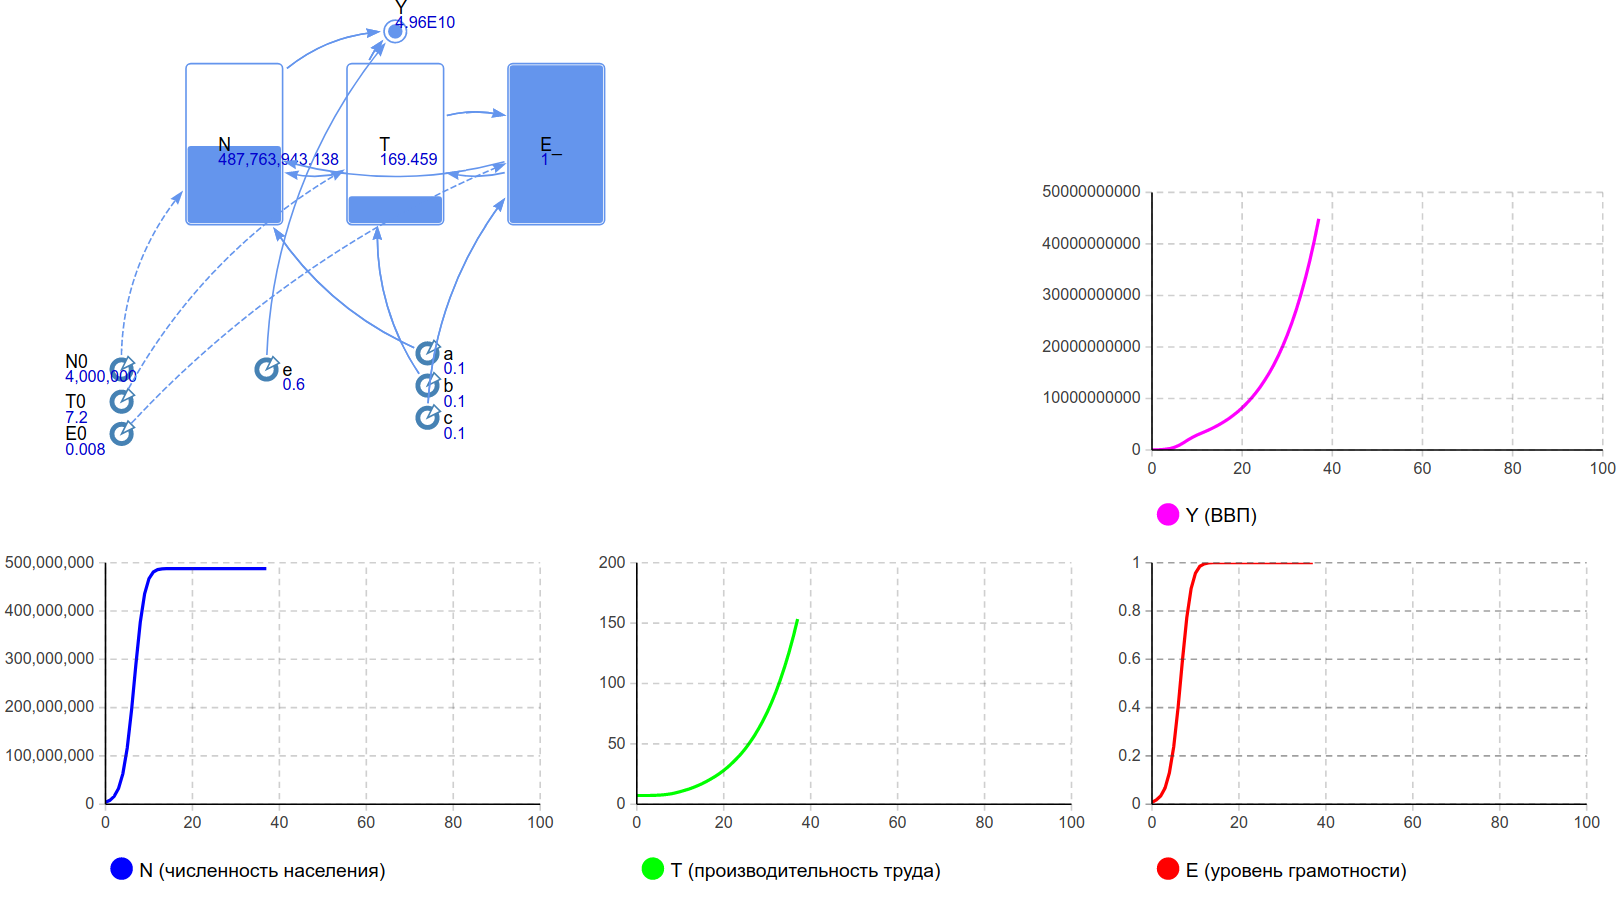
\includegraphics[scale=0.23]{korotaev1}
	\caption{Результаты построения модели Коротаева в AnyLogic с параметрами: $a = 0.1$, $b = 0.1$, $c = 0.1$ и $e = 0.6$}
	\label{fig:korotaev1}
\end{figure}

\newpage

Теперь попробуем поменять значения параметров: $a = 0.1$, $b = 0.1$, $c = 0.1$ и $e = 0.3$. (Рисунок \ref{fig:korotaev2})
\begin{figure}[h]
	\centering 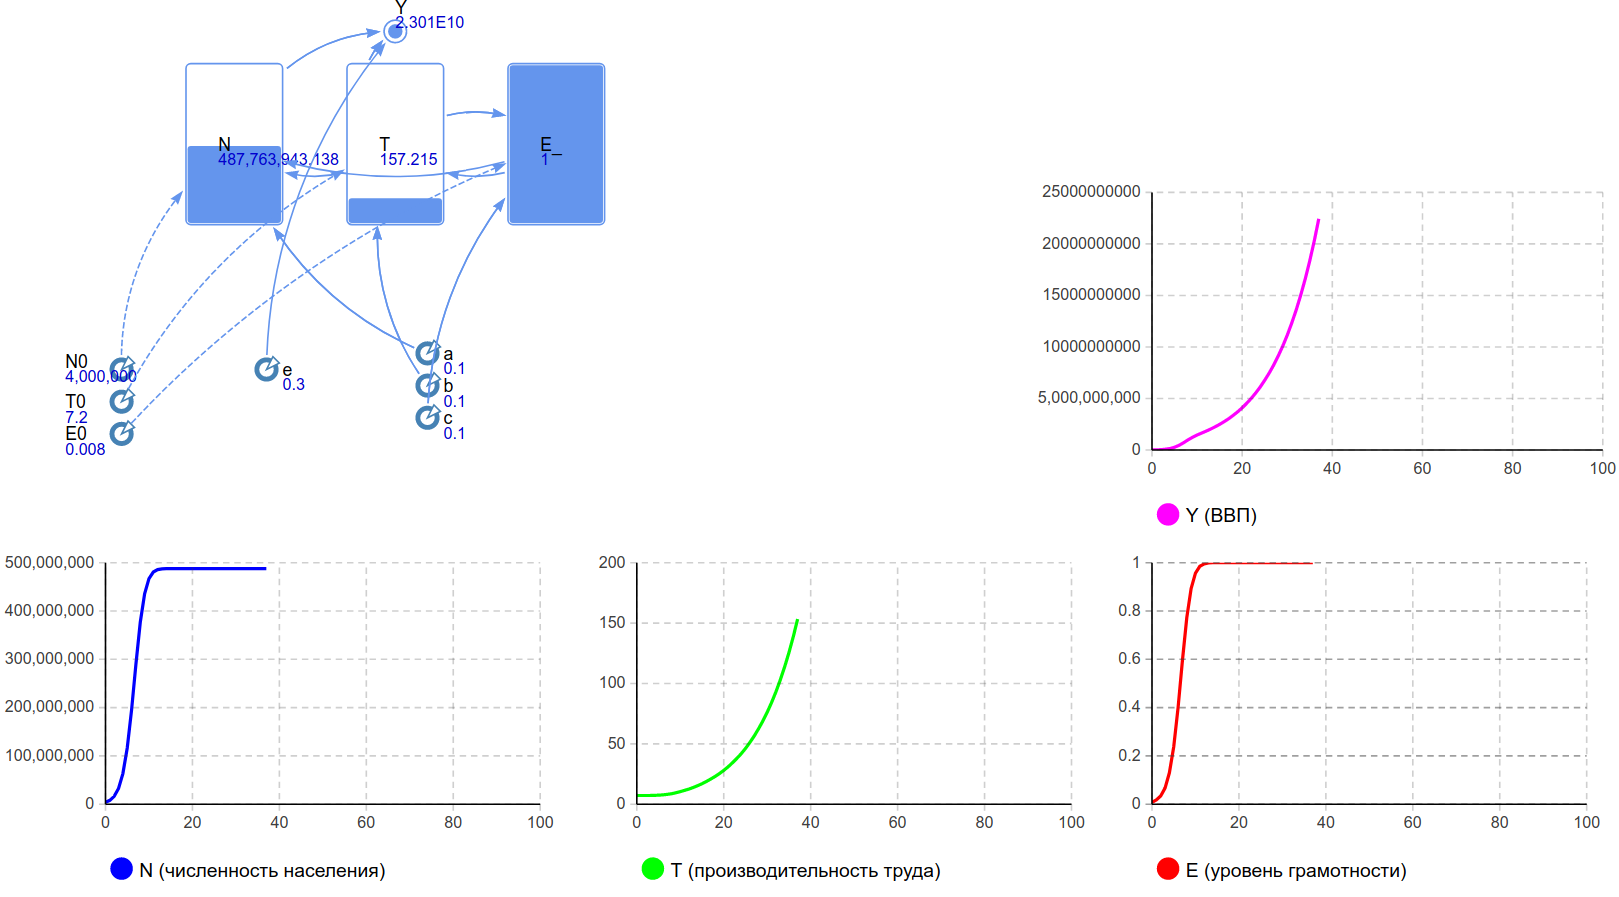
\includegraphics[scale=0.23]{korotaev2}
	\caption{Результаты построения модели Коротаева в AnyLogic с параметрами: $a = 0.1$, $b = 0.1$, $c = 0.1$ и $e = 0.3$}
	\label{fig:korotaev2}
\end{figure}

Можно видеть, что отношение числа работающего населения ко всему населению напрямую влияет на величину мирового ВВП, то есть чем меньше значение параметра $e$, тем меньше будет значение ВВП -- $Y$.

Теперь попробуем поменять значения параметров: $a = 0.1$, $b = 0.7$, $c = 0.1$ и $e = 0.3$. (Рисунок \ref{fig:korotaev3})
\begin{figure}[h]
	\centering 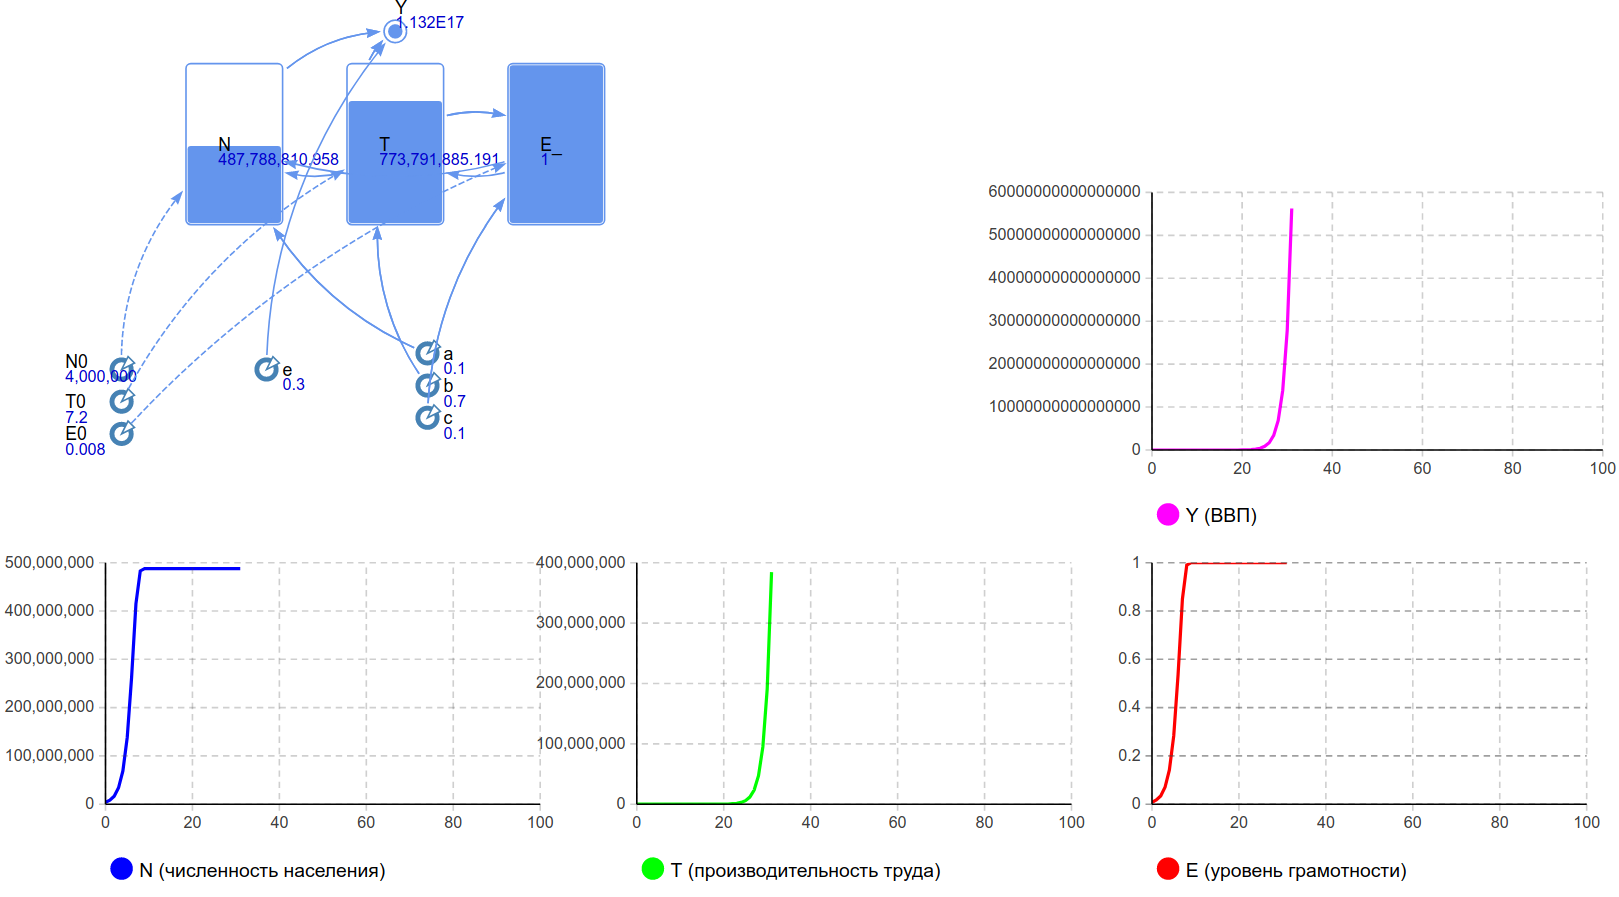
\includegraphics[scale=0.22]{korotaev3}
	\caption{Результаты построения модели Коротаева в AnyLogic с параметрами: $a = 0.1$, $b = 0.7$, $c = 0.1$ и $e = 0.3$}
	\label{fig:korotaev3}
\end{figure}

Можно видеть, что с увеличением значения $b$, растут значения $Y$ и $T$.\\

Таким образом, была реализована модель Коротаева при различных параметрах.